\section{Modello relazionale}
Nel senso stretto del termine, la \textit{relazione} di cui 
parla il modello è una relazione \textbf{matematica}; prendiamo 
la seguente tabella come esempio

\begin{center}
  \begin{tabular}{|l|r|}
    \hline
    a & 1 \\
    a & 2 \\
    b & 1 \\
    b & 2 \\
    \hline
  \end{tabular}
\end{center}

Questa è la tabella nata dal prodotto cartesiano di due 
due insiemi, \(D_1 = \{1, 2\} \) e \(D_2 = \{a, b\} \) e 
la relazione \(r\) sarà quindi solo parte di queste combinazioni,
quindi \( r \subseteq D_1 \times D_2\); per esempio
imponiamo che la nostra relazione sia 
\textit{"il numero corrispondente alla lettera"} : 

\begin{center}
    % Primo blocco (Tabella superiore nell'immagine)
    \begin{minipage}{0.3\textwidth}
        \centering
        \begin{tabular}{|c|c|}
            \hline
            a & 1 \\
            b & 2 \\
            \hline
        \end{tabular}
    \end{minipage}
    $\subseteq$ % Il simbolo di inclusione al centro
    % Secondo blocco (Tabella inferiore nell'immagine)
    \begin{minipage}{0.3\textwidth}
        \centering
        \begin{tabular}{|c|c|}
            \hline
            a & 1 \\
            a & 2 \\
            b & 1 \\
            b & 2 \\
            \hline
        \end{tabular}
    \end{minipage}
\end{center}

Proprio come nella matematica le due tabelle originali \(D_1\) e 
\(D_2\) saranno i \textbf{domini} della relazione.
\\
\\
Un elemento della relazione potrà quindi essere la d-upla 
\( (a, 1) \) e possiamo notare come la \textbf{posizione} degli elementi
all'interno della d-upla è molto importante, infatti sappiamo che
\(a\) viene dalla prima tabella e \(1\) dalla seconda.
La relazione sarà quindi un insieme di n-uple ordinate del tipo

\[ (d_1, d_2 \dots d_n) \quad | \quad 
d_1 \in D_1, d_2 \in D_2 \dots d_n \in D_n\]

Molto più diffuse sono invece le strutture \textbf{non posizionali},
ovvero quelle dove la posizione degli elementi della enn-upla non
ha importanza, questo perchè ogni elemento è invece appartenente ad
un \textbf{attributo}.

\begin{center}
  \begin{tabular}{|c|c|c|c|}
    \hline
    Casa & Fuori & RetiCasa & RetiFuori \\
    \hline
    Juve & Lazio & 3 & 1 \\
    Lazio & Milano & 0 & 1 \\
    Juve & Roma & 2 & 2 \\
    Roma & Milano & 0 & 3 \\
    \hline
  \end{tabular}
\end{center}

Come si vede in questo esempio ogni dominio ha desso un 
\textit{attributo} che descrive il suo scopo.
\\
\\
Dobbiamo specificare che il modello è basato su \textbf{valori},
ogni dato al suo interno sono valori, non abbiamo matrici,
array o addirittura puntatori, all'interno delle nostre
tabelle. Capiterà però che avremo bisogno di fare
\textbf{riferimento} a dati presenti in altre relazioni; voglio
inoltre specificare che in futuro vedremo più nel dettaglio
questo particolare caso ma per ora vediamo come viene 
"visualizzato" nelle tabelle.

\begin{center}
  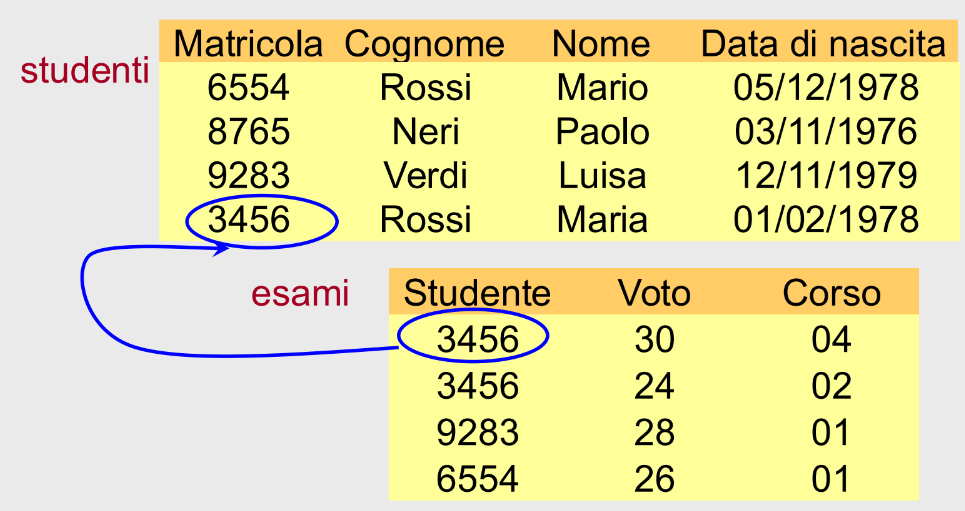
\includegraphics[width=0.8\textwidth]{modello relazionale/riferimento-tra-relazioni.png}
\end{center}

Come vediamo il valore della colonna \textit{Studente} nella
relazione \textit{esami} fa riferimento al valore all'interno
della colonna \textit{Matricola} nella relazione \textit{studenti}.
\\
\\
Poichè il modello usa valori ci servirà anche un \textbf{tipo} di
valore per rappresentare valori sconosciuti, inesistenti o senza 
informazione: useremo quindi il valore \textbf{NULL}.
Un altro caso molto comune è quello dove invece conosciamo il valore
ma deve rispettare dei \textbf{vincoli}, prendiamo come esempio 
la relazione \textit{esami} vista prima. \\
Il voto universtario \underline{deve} essere un intero compreso
tra 18 e 30, questo implica un \textbf{vincolo}. Infatti 
qualsiasi sia il modo di immettere dati all'interno del 
nostro database dovremo imporre un \textbf{vincolo d'integrità} e 
controllare che qualsiasi numero sia stato insierito rispetti questi
vincoli.
\\
\\
Andando più nello specifico l'esempio appena fatto fa parte 
di una serie di vincoli chiamati \textbf{vincoli intra-relazionali},
ovvero quei vincoli che interessano una tabella. \\
L'esempio sul voto è un \textbf{vincolo di dominio}, poichè tutto
il dominio dei voti deve rispettare quel vincolo, ma abbiamo anche il 
\textbf{vincolo di ennupla}, che invece interessano più valori della
stessa riga; per esempio se abbiamo la relazione \textit{stipendio}, 
che raccoglie lo stipendio dei lavoratori ogni mese e infine uno 
\textit{stipendio annuale}, quest'ultima colonna dovrà essere 
\underline{esattamente} la somma di ogni stipendio mensile. \\
Infine abbiamo un'altra categoria di vincoli, quelli \textbf{inter-razionali}
che interessano invece più relazioni; in questo caso semplicemente
il vincolo impone che se io faccio riferimento ad un dato di un'altra 
tabella quel dato \underbar{deve} esistere in quella tabella.
\\
\\
Identificare una riga all'interno di una tabella è molto importante,
potrebbe servirci capire quale riga crea problemi al database o 
potrebbe essere utile semplicemente cancellarla. Per questo motivo
esiste un altro \textit{vincolo indiretto}, quello della \textbf{chiave}.
Il vincolo impone infatti che ogni riga della tabella sia
\underline{diversa} dalle altre. Per essere tale basta che una 
enn-upla sia diversa dalle altre, anche di un solo valore. \\
L'insieme di dati che identificano una enn-upla prende il nome di 
\textbf{superchiave}.

\begin{center}
  \begin{tabular}{|c|c|c|c|}
    \hline
    Matricola & Nome & Cognome & Corso \\
    \hline
    12345 & Walter & Saitta & Ing. Informatica \\
    22234 & Federico & Bellomia & Ing. Edile \\
    90311 & Veronica & Ciulla & Psicologia \\
    04316 & Luca & Tigre & Architettura \\
    \hline
  \end{tabular}
\end{center}

In una tabela di questo tipo possiamo subito usare come 
\textit{superchiave} l'attributo \textbf{Matricola} poichè, per come 
è definita una matricola, non esisteranno due enn-uple con
matricole identiche; non solo, potremmo anche usare l'insieme di 
attributi (\textit{Matricola}, \textit{Nome}, \textit{Cognome}), 
con la stessa logica usata prima possiamo dire che non esisterà
altro studente con lo stesso nome, cognome e matricola di un altro. \\
C'è però una grossa distinzione tra le due, la 
prima (\textit{Matricola}) è infatti una \textbf{chiave}, 
ovvero il set di attributi \textbf{minimi} che identifica una 
riga della tabella; quindi ogni \textit{chiave} è anche una 
\textit{superchiave}, ma non è detto il contrario.